\documentclass[10pt]{article}

\usepackage[margin=0.75in]{geometry}
\usepackage{graphicx}
\usepackage{amsmath}
\usepackage{listings}
\usepackage{float}
\usepackage{fancyhdr}
\pagestyle{fancy}
\begin{document}
\rhead{Chris Larson}
Chris Larson
HW11

\begin{lstlisting}
==================================================
==================================================
==================================================
library ieee;
use ieee.std_logic_1164.all;

entity xor2 is
port(A, B : in std_logic;
     Y : out std_logic);
end xor2;

architecture df of xor2 is
begin
	Y <= A XOR B;
end;
==================================================
==================================================
==================================================
library ieee;
use ieee.std_logic_1164.all;

entity full_adder is 
	port(A , B, Cin : in std_logic;
	     Sum, Cout : out std_logic);
	end full_adder;

architecture struct of full_adder is
	component xor3 is 
	port (A, B, C : in std_logic;
	      Y : out std_logic);
	end component;

	component and2 is 
	port(A, B : in std_logic;
	     Y : out std_logic);
	end component;
	
	component or3 is 
	port(A, B, C : in std_logic;
	     Y : out std_logic);
	end component;
	
	signal s_1, s_2, s_3 : std_logic:='0';
begin
	xor3_instance1 : xor3 port map (A => A , B => B, C => Cin, Y => Sum);

	and2_instance1 : and2 port map (A => A,  B => B, Y => s_1); 
	and2_instance2 : and2 port map (A => A,  B => Cin, Y => s_2); 
	and2_instance3 : and2 port map (A => Cin,  B => B, Y => s_3);

	or3_instance1 : or3 port map (A => s_1, B => s_2, C => s_3, Y => Cout);

end;
==================================================
==================================================
==================================================
library ieee;
use ieee.std_logic_1164.all;

entity and2 is
port(A, B : in std_logic;
     Y : out std_logic);
end and2;

architecture df of and2 is
begin
	Y <= A AND B;
end;
==================================================
==================================================
==================================================
library ieee;
use ieee.std_logic_1164.all;

entity xor3 is
port(A, B, C : in std_logic;
     Y : out std_logic);
end xor3;

architecture df of xor3 is
begin
	Y <= A XOR B XOR C;
end;
==================================================
==================================================
==================================================
library ieee;
use ieee.std_logic_1164.all;

entity or3 is
port(A, B, C : in std_logic;
     Y : out std_logic);
end or3;

architecture df of or3 is
begin
	Y <= A OR B OR C;
end;
==================================================
==================================================
==================================================
library ieee;
use ieee.std_logic_1164.all;

entity four_bit is
	port(Y1, Y2, Y3, Y4, A_S : in std_logic;
	     X1, X2, X3, X4 : in std_logic;
	     S1, S2, S3, S4, Cout : out std_logic);
end four_bit;

architecture struct of four_bit is
	component xor2 is
		port (A, B : in std_logic;
		      Y : out std_logic);
	end component;

	component full_adder is 
		port(A, B, Cin : in std_logic;
		     Sum, Cout : out std_logic);
	end component;

	signal s_1, s_2, s_3, s_4, s_5, s_6, s_7 : std_logic := '0';

begin
	xor2_instance1 : xor2 port map (A => A_S, B => Y1, Y => s_1); 
	xor2_instance2 : xor2 port map (A => A_S, B => Y2, Y => s_2);
	xor2_instance3 : xor2 port map (A => A_S, B => Y3, Y => s_3);
	xor2_instance4 : xor2 port map (A => A_S, B => Y4, Y => s_4);
	
	full_adder_instance1 : full_adder port map (A => s_1, B => X1, Cin => A_S,
								 Cout => s_5, Sum => S1);
	full_adder_instance2 : full_adder port map (A => s_2, B => X2, Cin => s_5,
								 Cout => s_6, Sum => S2);
	full_adder_instance3 : full_adder port map (A => s_3, B => X3, Cin => s_6,
								 Cout => s_7, Sum => S3);
	full_adder_instance4 : full_adder port map (A => s_4, B => X4, Cin => s_7,
								 Cout => Cout, Sum => S4);
end;
==================================================
==================================================
==================================================
library ieee;
use ieee.std_logic_1164.all;
use ieee.std_logic_unsigned.all;

entity tb is
end tb;

architecture behv of tb is 
	component four_bit is
	port(Y1, Y2, Y3, Y4, A_S : in std_logic;
	     X1, X2, X3, X4 : in std_logic;
	     S1, S2, S3, S4, Cout : out std_logic);
	end component;

signal aY1 : std_logic := '0';
signal aY2 : std_logic := '0';
signal aY3 : std_logic := '0';
signal aY4 : std_logic := '0';
signal aX1 : std_logic := '0';
signal aX2 : std_logic := '0';
signal aX3 : std_logic := '0';
signal aX4 : std_logic := '0';
signal aS1 : std_logic := '0';
signal aS2 : std_logic := '0';
signal aS3 : std_logic := '0';
signal aS4 : std_logic := '0';
signal aCout : std_logic := '0';
signal aA_S : std_logic := '0';

for UUT : four_bit use entity work.four_bit(struct);
begin 

	UUT : four_bit port map (Y1 => aY1, Y2 => aY2, Y3 => aY3, Y4 => aY4,
				 X1 => aX1, X2 => aX2, X3 => aX3, X4 => aX4, 
				 A_S => aA_S, S1 => aS1, S2 => aS2, S3 => aS3,
				  S4 => aS4, Cout => aCout);

process
begin
	aY1 <= '1';
	aY2 <= '0';
	aY3 <= '1';
	aY4 <= '0';
	aX1 <= '0';
	aX2 <= '1';
	aX3 <= '0';
	aX4 <= '1';
	aA_S <= '0';
	wait for 50 ns;

	aY1 <= '1';
	aY2 <= '1';
	aY3 <= '0';
	aY4 <= '0';
	aX1 <= '0';
	aX2 <= '1';
	aX3 <= '0';
	aX4 <= '1';
	aA_S <= '0';
	wait for 50 ns;

	aY1 <= '1';
	aY2 <= '1';
	aY3 <= '1';
	aY4 <= '1';
	aX1 <= '1';
	aX2 <= '1';
	aX3 <= '1';
	aX4 <= '1';
	aA_S <= '0';
	wait for 50 ns;

	aY1 <= '1';
	aY2 <= '1';
	aY3 <= '0';
	aY4 <= '0';
	aX1 <= '1';
	aX2 <= '1';
	aX3 <= '1';
	aX4 <= '0';
	aA_S <= '1';
	wait for 50 ns;
	
	aY1 <= '1';
	aY2 <= '1';
	aY3 <= '0';
	aY4 <= '0';
	aX1 <= '0';
	aX2 <= '1';
	aX3 <= '0';
	aX4 <= '1';
	aA_S <= '1';
	wait for 50 ns;
	
	aY1 <= '0';
	aY2 <= '1';
	aY3 <= '0';
	aY4 <= '1';
	aX1 <= '1';
	aX2 <= '0';
	aX3 <= '1';
	aX4 <= '0';
	aA_S <= '1';
	wait for 50 ns;
end process;
end;
\end{lstlisting}

\begin{figure}[H]
	\centering
	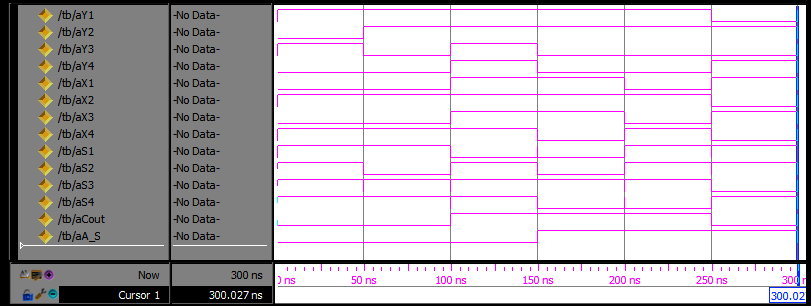
\includegraphics[width=1\textwidth]{ModelSimHW11PT2}
	\caption{HW11 Simulation results}
	\label{fig:Figure 1}
\end{figure}

\begin{table}[H]
	\centering
	\caption{PART II TABLE}
	\label{tab:Table 1}
	\begin{tabular}{|c|c|c|c|c|}
		\hline
		A3 A2 A1 A0 & B3 B2 B1 B0 & C4 & F3 F2 F1 F0 & A + B = F \\ \hline
		X4 X3 X2 X1 & Y4 Y3 Y2 Y1 & Cout & S4 S3 S2 S1 & (decimal)\\ \hline
		1 0 1 0 & 0 1 0 1 & 0 & 1 1 1 1 & (-6) + 5 = -1 \\ \hline
		1 0 1 0 & 0 0 1 1 & 1 & 1 1 0 1 & (-6) + 3 = -3 \\ \hline
		1 1 1 1 & 1 1 1 1 & 1 & 1 1 1 0 & (-1) + (-1) = -2 \\ \hline
		0 1 1 1 & 0 0 1 1 & 0 & 0 1 0 0 & 7 + 3 = 4 \\ \hline
		1 0 1 0 & 0 0 1 1 & 1 & 0 1 1 1 & (-6) - 3 = -9 \\ \hline
		0 1 0 1 & 1 0 1 0 & 0 & 1 0 1 1 & 5 - (-6) = 11 \\ \hline
	\end{tabular}
\end{table}

\end{document}